\section{Background}
\label{sec:background}

Collaborative-filtering is a recommendation approach that uses similarity between users and the benefit they have received from items in the past to make recommendations. Three main approaches to collaborative filtering are memory-based, model-based and hybrid methods~\cite{Su:2009:SCF:1592474.1722966} . Memory-based approaches, specifically item-based recommender~\ref{fig:predict}, use an item-user rating matrix to compute pairwise similarities between items. In the contexts of courses, enrollment roster, previous courses students taken and grades course give, is a natural way to reason about course similarity.  

\begin{figure}[h]
 \centering % avoid the use of \begin{center}...\end{center} and use \centering instead (more compact)
 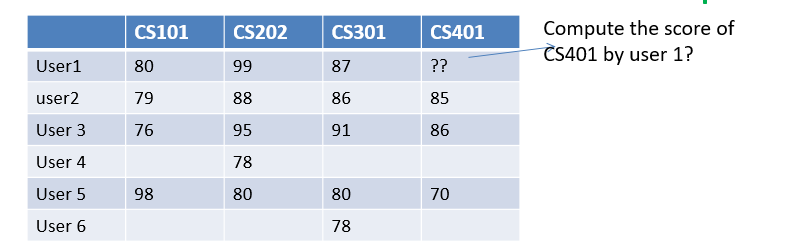
\includegraphics[width=\linewidth]{figs/predict}
 \caption{Typical student course grade table}
 \label{fig:predict}
\end{figure}

However the recommendation approaches are not appropriate for our problems, since they are used for making predictions which means, the approach is designed to fill in the missing values in the matrix. For our case, however, we want to figure out how two courses are correlated with each other. We don’t want to fill the matrix since it will blur the original data. What’ more, for each two courses we are only interested in the users who take both of them. Visualization is an effective and intuitive way to approach our goal.  

There’re many existing similarity measures to compare two entities. Well known metrics include Euclidean similarity, Jaccard(Tanimoto) similarity, Pearson Correlation Coefficient, cosine similarity and Log-likelihood similarity etc. Euclidean similarity measures the distance between courses grading vectors. Jaccard(Tanimoto) similarity is calculated by dividing the intersection of the sets by the union of those sets\cite{sandvig2005aacorn}. Cosine Similarity envision user’s ratings as points in space and measures the cosine of the angle between these lines drawn from origin to each point. The Log-likelihood similarity is a measure of how often items from 2 sets appear together versus how often they appear apart. Pearson Correlation Coefficient is a number between -1, 1. It measures the tendency of the rating vectors, paired one by one, and it’s typically used in early research papers. Its formula is given as $pearson-correlation(u,w) = \frac{cov(R_u,R_w)}{\sigma x \sigma y} $ where $cov$ stands for covariance and $\sigma x$ stands for standard deviation of $x$. We are interested in the strong positive correlation and the positive correlation as illustrated in~\ref{fig:psc}.

For our work, Euclidean similarity is not suitable because courses taken by more students will be added more distances. Jaccard(Tanimoto) similarity and Log-likelihood don’t count grades students get. We choose Pearson Correlation coefficient to indicate the similarity between two courses and based on that, we build our item-based recommender system and provide a way to measure the benefits between two courses.
\begin{figure}[h]
 \centering % avoid the use of \begin{center}...\end{center} and use \centering instead (more compact)
 \includegraphics[width=1.5in]{figs/psc_illustrated}
\caption{Pearson Correlation Illustrated}
 \label{fig:psc}
\end{figure}


